\documentclass[conference]{IEEEtran}
% CANOPIE-HPC @ SC26 submission (IEEE proceedings format). Draft.
\IEEEoverridecommandlockouts

\usepackage{cite}
\usepackage{amsmath}
\usepackage{graphicx}
\usepackage{booktabs}
\usepackage{multirow}
\usepackage{url}
\usepackage[T1]{fontenc}
\usepackage{tikz}
\usetikzlibrary{arrows.meta, positioning}
\usepackage[ruled,vlined]{algorithm2e}

\begin{document}

\title{A Polite, Container-Native Bursting Fabric for AI Workloads on Shared Clusters}

\author{\IEEEauthorblockN{Andrew H. Bond}
\IEEEauthorblockA{San Jos\'e State University\\
San Jos\'e, CA, USA\\
andrew.bond@sjsu.edu\\
ORCID: \texttt{0009-0003-2599-6158}}}

\maketitle

\begin{abstract}
Turning a shared, multi-tenant GPU cluster into elastic capacity means fighting
\texttt{kubectl}, YAML, and container cold starts, with no feedback loop into running code. We
present a \emph{polite, container-native bursting fabric} that makes cluster GPUs appear as elastic
capacity \emph{inside the user's program}. The fabric, \textbf{nats-bursting}, makes cluster pods
first-class subscribers on the same NATS bus as the workstation---as ephemeral Kubernetes Jobs or
persistent queue-group pools---behind a Go control plane whose \emph{politeness controller} probes
cluster state and backs off rather than crowding tenants. Its leaf-node topology surfaces
orchestration issues (JetStream vs.\ core-NATS delivery, asymmetric subject interest). Two
components make bursting practical: \textbf{turboquant-pro} compresses on-wire payloads, and
\textbf{batch-probe} right-sizes each pod's GPU batch. We measure it on real
infrastructure---burst cold-start $\sim$6.6\,s, warm pool $\sim$67\,ms, up to $8.4\times$
compression speedup over a $\sim$2\,Mbps link, 94\% GPU utilization---and release all three
projects and the harness.
\end{abstract}

\begin{IEEEkeywords}
cloud bursting, Kubernetes, containers, orchestration, NATS, NRP Nautilus, vector quantization,
KV-cache compression, GPU utilization, thermal control
\end{IEEEkeywords}

\section{Introduction}
Shared, multi-tenant Kubernetes clusters such as NRP Nautilus~\cite{nautilus} exist precisely so
that researchers without their own datacenter can burst. Yet ``use the cluster from my
workstation'' remains awkward: one writes Kubernetes manifests, submits Jobs, polls for
completion, and shuttles data in and out---none of it inside the program where the research runs.
The friction is high enough that elastic capacity often goes unused.

Consider a concrete case. A researcher iterating on an embedding or inference pipeline at their
workstation wants, for one hour, to fan ten thousand documents across a dozen cluster GPUs, then
return to interactive work. Today that means authoring a Job manifest, building and pushing a
container image, submitting, polling, and copying results back---a context switch out of the
program and into cluster operations. The capability exists; the ergonomics do not. And on a
\emph{shared} cluster a second obligation rides along: a convenience layer must not crowd out the
other tenants, or it will (rightly) get its owner throttled or banned.

This paper describes a polite, container-native \emph{bursting fabric} that closes the gap while
honoring that obligation, and measures it honestly on the real cluster. Its core is the fabric
itself; two supporting components make remote bursting practical:

\begin{itemize}
\item \textbf{The bursting fabric} (nats-bursting, \S\ref{sec:bursting})---the primary
contribution: a Go control plane plus a Python client that make containerized cluster pods
\emph{first-class subscribers} on the researcher's own NATS bus, in two shapes (ephemeral Jobs,
persistent pools), behind a \emph{politeness controller} that probes cluster state and backs off
to yield to other tenants. Its NATS leaf-node topology surfaces concrete orchestration design
tradeoffs (JetStream vs.\ core-NATS delivery, asymmetric subject interest) we report as an
experience.
\item \textbf{Transport optimization} (turboquant-pro, \S\ref{sec:tq})---compressing bus payloads
so remote bursting stays viable over constrained links, reported at the level a practitioner
needs: ratios, fidelity, real-link speedup, and a rule for \emph{when} compression helps.
\item \textbf{Resource management} (batch-probe, \S\ref{sec:bp})---right-sizing each pod's GPU
batch (and thermally governing the local driver) so bursts remain useful and within a shared
cluster's utilization policy.
\end{itemize}

We then quantify the fabric on real infrastructure (\S\ref{sec:eval}), state threats to validity
(\S\ref{sec:threats}), and reflect on the engineering (\S\ref{sec:discussion}). This is a
practice/experience paper: a working, open system plus measurements. Its value is the
orchestration design---particularly the politeness controller that makes ``effective and
policy-safe'' mechanical rather than aspirational---and the honest characterization of when each
supporting layer helps.

\textbf{Why SC.} This is a systems paper about operationalizing opportunistic, shared GPU capacity
for AI workloads. The contribution is not a new scheduler or a new quantizer, but a
\emph{policy-aware bursting fabric} that turns multi-tenant Kubernetes GPUs into
event-loop-local capacity, with reproducible measurements of cold start, warm-pool latency,
compressed transport, admission control under contention, and GPU utilization.

\section{Background}
\textbf{NRP Nautilus}~\cite{nautilus} is a shared, opportunistic Kubernetes cluster. Its usage
policy shapes the design: small/idle pods are tolerated (CPU\,$\le$\,1, mem\,$\le$\,2\,GiB are an
``ignored'' range), but groups of pods must sustain utilization (5+ pods must each stay under
40\% GPU), Jobs must run to completion and exit cleanly (no \texttt{sleep}-camping), and requests
should match usage. ``Effective and policy-safe'' is therefore a container-orchestration design
target, not a slogan.

\textbf{NATS}~\cite{nats} provides subject-based publish/subscribe and request--reply; \emph{queue
groups} that round-robin a subject across a set of subscribers; \emph{JetStream}, a persistence
layer with work-queue streams and durable pull consumers (at-least-once, redelivery); and
\emph{leaf nodes} that bridge a remote NATS server into a hub. Leaf-node federation is central to
our design and to two of its sharper engineering decisions (\S\ref{sec:bursting}): JetStream is
not federated across a leaf link, and subject \emph{interest} can propagate asymmetrically
hub$\to$spoke.

\textbf{Cloud bursting} spills work from a local resource to a remote one. We use a message bus
rather than a job queue or RPC because it makes the containerized cluster a \emph{peer} on the
fabric the application already speaks, so a burst becomes a publish inside the event loop.

\section{nats-bursting: the bursting fabric}\label{sec:bursting}

\begin{figure}[t]\centering
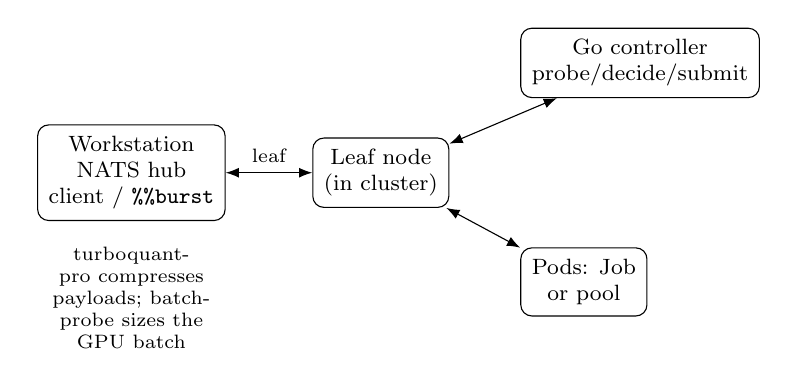
\begin{tikzpicture}[
  box/.style={draw, rounded corners, align=center, font=\footnotesize, inner sep=4pt},
  >=Latex]
\node[box] (ws) {Workstation\\ NATS hub\\ client / \texttt{\%\%burst}};
\node[box, right=11mm of ws] (leaf) {Leaf node\\ (in cluster)};
\node[box, above right=5mm and 9mm of leaf] (ctl) {Go controller\\ probe/decide/submit};
\node[box, below right=5mm and 9mm of leaf] (pods) {Pods: Job\\ or pool};
\draw[<->] (ws) -- node[above, font=\scriptsize]{leaf} (leaf);
\draw[<->] (leaf) -- (ctl);
\draw[<->] (leaf) -- (pods);
\node[font=\scriptsize, text width=24mm, align=center, below=2mm of ws]
  {turboquant-pro compresses payloads; batch-probe sizes the GPU batch};
\end{tikzpicture}
\caption{Two shapes, one bus. Ephemeral bursts go workstation$\to$Go controller$\to$Kubernetes
Job; persistent pools are queue-group worker Deployments the client dispatches to directly. Both
reach the workstation over an outbound leaf link.}\label{fig:arch}
\end{figure}

nats-bursting has two halves joined by one bus (Fig.~\ref{fig:arch}): a Go control plane that
lives next to the cluster and turns NATS messages into Kubernetes objects, and a Python client
used from notebooks and scripts. Two workload \emph{shapes} share the bus but use different
control paths.

\subsection{The control plane and its politeness controller}
The Go controller is event-driven. Its \texttt{natsbridge} subscribes to \texttt{burst.submit},
and on each request the \texttt{submitter} renders a \texttt{JobDescriptor} into a real
\texttt{batchv1.Job} via client-go---CPU/memory/\texttt{nvidia.com/gpu}/ephemeral-storage requests
and limits, a managed-by label, \texttt{RestartPolicyNever}, and foreground-propagation
cancellation---then publishes a status event. The wire protocol is three subject families:
\texttt{burst.submit} (requests), \texttt{burst.status.\textless job\textgreater} (a
\texttt{submitted}/\texttt{error} state machine), and \texttt{burst.result.\textless
job\textgreater} (reserved for results). The client issues a request--reply on
\texttt{burst.submit} and falls back to subscribing on the status subject---robust to whichever
pattern the controller answers with.

The part the rest of this paper's ``policy-safe'' claim rests on is the \emph{politeness
controller}. A \texttt{prober} reads live cluster state through client-go---total/allocated/idle
nodes, the caller's own running and pending Jobs, \emph{and other tenants' pending pods}---and
degrades gracefully when an individual API call is denied by RBAC. A \texttt{decider} then
evaluates that state against thresholds in a fixed priority order: (1)~\emph{self-limiting}---do
not exceed your own running/pending caps (defaults 50/20); (2)~\emph{courtesy}---yield when more
than a threshold of \emph{other} users' pods are queued (default 200); (3)~\emph{utilization}---back
off when cluster allocation exceeds a fraction (default 0.90). The outcome is
\texttt{Submit}/\texttt{Backoff}/\texttt{Abort} (Algorithm~\ref{alg:polite}, with thresholds in
Table~\ref{tab:cfg}). Backoff is capped exponential with jitter applied \emph{after} the cap,
\begin{equation}
w_k \;=\; \min\!\bigl(B_0\,m^{\,k},\,B_{\max}\bigr)\cdot\Bigl(1 + \tfrac12\bigl(u-\tfrac12\bigr)\Bigr),
\quad u\sim\mathcal U[0,1),
\end{equation}
i.e.\ $\pm$25\% jitter to decorrelate wake-ups across many controllers (anti-thundering-herd),
aborting after $K$ attempts. This is what makes ``yield to other tenants'' a mechanism rather than
a promise: the system measures the shared cluster and defers to it.

\begin{algorithm}[t]
\caption{Polite admission decision}\label{alg:polite}
\KwIn{cluster state $s$ (from the prober), thresholds $p$}
\KwOut{\texttt{Submit} / \texttt{Backoff} / \texttt{Abort}}
\lIf{$\mathrm{attempts}\ge p.\mathrm{maxAttempts}$}{\Return \texttt{Abort}}
\lIf{$s.\mathrm{myRunning}\ge p.\mathrm{maxConcurrent}$}{\Return \texttt{Backoff}}
\lIf{$s.\mathrm{myPending}\ge p.\mathrm{maxPending}$}{\Return \texttt{Backoff}}
\lIf{$s.\mathrm{othersPending}> p.\mathrm{queueDepth}$}{\Return \texttt{Backoff}}
\lIf{$s.\mathrm{alloc}/s.\mathrm{total}> p.\mathrm{util}$}{\Return \texttt{Backoff}}
\Return \texttt{Submit}\;
\end{algorithm}

\begin{table}[t]\centering\caption{Politeness controller defaults.}\label{tab:cfg}
\begin{tabular}{lr}\toprule
parameter & default \\\midrule
max concurrent jobs (self-limit) & 50 \\
max pending jobs (self-limit) & 20 \\
others-pending threshold (courtesy) & 200 \\
utilization threshold (load) & 0.90 \\
initial / max backoff & 30\,s / 30\,min \\
backoff multiplier / max attempts & 2.0 / 20 \\\bottomrule
\end{tabular}
\end{table}

\subsection{The Python client and the \texttt{\%\%burst} magic}
The client is a synchronous facade over async NATS, owning one background event loop and a
\texttt{Transport} seam for deterministic testing. \texttt{JobDescriptor}/\texttt{Resources}
mirror the Go structs field-for-field. A \texttt{\%\%burst} IPython cell magic makes a burst an
editor action: by default (\texttt{--when-busy}) it probes the local GPUs through
\texttt{nvidia-smi} and only offloads when every local GPU is saturated, otherwise running the
cell in place; \texttt{--always}/\texttt{--never} force the choice, and \texttt{--gpu/--cpu/--image}
set resources. The cell body is shipped as an environment variable and executed in the pod, so
no image rebuild is needed for ad-hoc work.

\subsection{Persistent pools, queue groups, and leaf federation}
The second shape is a persistent pool: a Deployment of always-on workers that subscribe as a NATS
queue group and stay warm (no per-task cold start, cached models). A \texttt{TaskDispatcher}
submits many tasks and collects results on \texttt{results.\textgreater}. Two delivery models
coexist, and the choice is a deliberate accommodation of leaf-node topology. With
\texttt{durable=True}, tasks go through a JetStream work-queue stream consumed by a durable pull
consumer shared across replicas (at-least-once, explicit ack/nak, bounded redelivery)---correct
when dispatcher and workers share a JetStream domain. With \texttt{durable=False}, tasks use core
NATS queue groups, which cross leaf-node boundaries that JetStream does not. A symmetric subtlety
appears on the return path: where subject interest propagates only hub$\to$spoke, results
published spoke-side never reach the hub, so the worker can optionally POST results to a webhook
that re-publishes them on the hub. The pool's defaults are NRP-quota-aware
(\texttt{cpu=1/mem=2Gi} to stay in the ``ignored'' swarm range), and the worker blocks inside
\texttt{fetch()} rather than sleeping---satisfying the ``no sleeping Jobs'' rule---with an
idle-exit watchdog that lets the same image run as either a Deployment (run forever) or a
self-terminating Job (exit after idle). These are small decisions, but each is the difference
between a demo and something that survives contact with a real multi-tenant cluster.

\section{Transport: making bursting viable over constrained links}\label{sec:tq}
When work bursts to a remote cluster, the payloads---embeddings, KV-cache pages, feature
tensors---ride the bus, and on a constrained link they, not the cluster, become the bottleneck
(\S\ref{sec:eval}). turboquant-pro compresses them so remote bursting stays viable; we report only
what a deployer needs, not the codec's internals.

\textbf{A distribution-free codec.} Each vector is L2-normalized, rotated by a shared,
seed-deterministic random rotation, and each rotated coordinate is quantized against a fixed
Lloyd--Max codebook and bit-packed. The rotation is the trick: by concentration of measure it
makes the coordinates approximately i.i.d.\ Gaussian \emph{regardless of the input
distribution}~\cite{turboquant}, so one fixed codebook is near-optimal for any data with no
training or calibration. The NATS codec frames each embedding as an 8-byte header (version, bits,
dim, norm) plus $\lceil\text{dim}\cdot\text{bits}/8\rceil$ packed bytes; the same construction
serves KV-cache \emph{values}, while \emph{keys}---whose error the softmax amplifies---instead use a
per-channel scheme (per-vector normalization is near-lossless for values but catastrophic for keys),
and values support attention computed directly on the compressed
codes~\cite{onlinesoftmax,flashattention}, though that kernel-level work is out of scope here.

\textbf{What a deployer needs.} Compression is $8$--$16\times$ at $4/3/2$ bits with reconstruction
cosine $0.94$--$0.995$, and is \emph{distribution-agnostic}---real transformer embeddings reproduce
the random-vector numbers to within 0.001 (\S\ref{sec:eval}). The deployment rule is simple and we
evidence it: \emph{compress when the link or bus is the bottleneck}. On a fast LAN it is a wash; on
a real $\sim$2\,Mbps link it cuts NATS round-trip up to $8.4\times$ for large payloads
(\S\ref{sec:eval}). Encode/decode are cheap relative to a constrained link but not free, so the
rule---not a blanket ``always compress''---is what we recommend.

\section{Resource management: keeping pods useful and policy-aligned}\label{sec:bp}
A burst is only worth its slot if each pod actually fills its GPU---a shared cluster rewards high
utilization and penalizes hoarding---and only sustainable if the node driving the burst does not
overheat. batch-probe provides both, as a support mechanism for the fabric.

\subsection{OOM-safe batch right-sizing}
\texttt{probe\_batch\_size} binary-searches the largest batch that fits, building inputs through a
caller-supplied \texttt{input\_fn(b)} and running a trial at each candidate. In \emph{infer} mode
the trial is a forward pass under \texttt{no\_grad}; in \emph{train} mode it instantiates an AdamW
optimizer and runs a full forward/backward/step, so the search reflects \emph{true} peak training
memory including optimizer moments---a detail most batch finders miss and under-estimate by
roughly the optimizer-state factor. OOM is caught and distinguished from genuine errors by message
inspection; an unconditional \texttt{finally} block deletes trial tensors and flushes the
allocator before the next iteration, which is what keeps the search stable across repeated OOMs
(Algorithm~\ref{alg:probe}). Headroom is a multiplicative shrink of the largest success
(default 0.8$\times$).

\begin{algorithm}[t]
\caption{OOM-safe batch right-sizing (infer mode)}\label{alg:probe}
\KwIn{model $M$, \texttt{input\_fn}, range $[\mathrm{lo},\mathrm{hi}]$, headroom $h$}
$best \gets 0$\;
\While{$\mathrm{lo}\le\mathrm{hi}$}{
  $b \gets \lfloor(\mathrm{lo}+\mathrm{hi})/2\rfloor$;\ \ cleanup()\;
  $ok \gets$ forward$\bigl(M,\texttt{input\_fn}(b)\bigr)$ completes without OOM\;
  free trial tensors;\ \ cleanup() \tcp*{unconditional: release fragments}
  \lIf{$ok$}{$best\gets b$;\ $\mathrm{lo}\gets b{+}1$}
  \lElse{$\mathrm{hi}\gets b{-}1$}
}
\Return $\max\!\bigl(1,\lfloor best\,(1-h)\rfloor\bigr)$\;
\end{algorithm} A generic
\texttt{probe(work\_fn)} extends the same recovery to any framework (Torch/CuPy/JAX) by abstracting
the memory-pool flush.

\subsection{Thermal-aware throttling}
On the local orchestration side, \texttt{ThermalController} keeps the workstation driving a burst
within a thermal budget. Rather than a fixed temperature threshold, it estimates thermal state
with a two-state Kalman filter~\cite{kalman} (temperature and its rate) and acts on the
\emph{predicted} trajectory: when it forecasts an overshoot within a short horizon it throttles
worker-thread count \emph{before} the limit is reached, using the filter's rate estimate as a clean
derivative. The same temperature oracle backs a one-shot thread-capacity search and an
admission-gating job manager. We keep this brief deliberately---it is a support mechanism here, not
the contribution---and note that thermal sensing is currently Linux-only.

\section{Evaluation}\label{sec:eval}
We evaluate the fabric in three tiers by the infrastructure each needs, plus the GPU-sizing
demonstration. Every number below is \emph{our own} measurement, reproducible from the released
harness (\S\ref{sec:artifact}); we do not re-run the supporting projects' internal benchmarks, and
report only what bears on the bursting use case.

\textbf{Experimental setup.} The workstation is a remote client. The on-premises node (``Atlas'')
has two NVIDIA GV100 32\,GB GPUs; it runs the NATS hub and the Tier-1/2 measurements. The shared
cluster is NRP Nautilus (namespace \texttt{ssu-atlas-ai}), reached from Atlas via \texttt{kubectl},
with a leaf-node pod bridging the cluster to the hub. The Tier-2 ``real hop'' traverses a
wide-area overlay link ($\sim$90\,ms RTT, $\sim$2\,Mbps effective). All cluster runs use
ignored-range pods (CPU\,$=$\,1, mem\,$=$\,2\,GiB) and at most four concurrent pods, to stay within
policy.

\textbf{Measurement protocol.} Latencies are p50/p99 over 40--500 requests after warm-up;
throughput is the wall-clock rate over the batch. Tier-2 round-trips are timed on the requesting
host with a single clock; for the real hop the responder runs on Atlas and the requester on the
remote workstation with \emph{no} co-located subscriber, so every request crosses the wire. Tier-3
cold-start is timed from Job submission to the Job's completion condition, with the
schedule$\to$container-start split read from the pod's own Kubernetes timestamps. Codec
encode/decode is timed in isolation (Tier~1) and excluded from the transport loop.

\subsection{Compression (Tier 1)}
On dim-1024 vectors the codec gives ratios of $7.9/10.4/15.5\times$ at $4/3/2$-bit with
reconstruction cosine $0.995/0.978/0.94$ (Fig.~\ref{fig:t1}). Re-running on real
\texttt{bge-small-en-v1.5} embeddings (20newsgroups, $n{=}3000$, native dim 384) gives
\emph{identical} ratio and cosine within 0.001 at matched dimension---confirming the
distribution-agnostic property empirically. The analytic transfer model follows: a 1\,MB batch
moves in $\sim$84\,ms at 100\,Mbps but $\sim$8\,ms compressed (a $\sim$63\,ms net saving after
encode) and is a wash at 1\,Gbps---the hypothesis Tier~2 tests. Cosine is a fidelity proxy, not a
downstream-task guarantee.

\begin{figure}[t]\centering
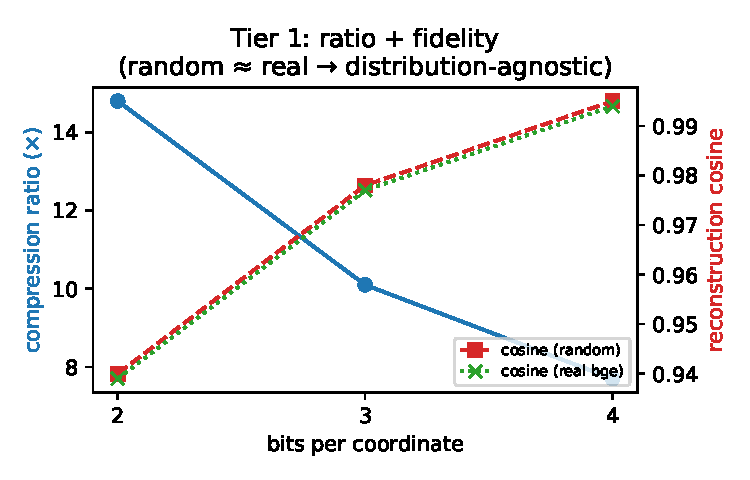
\includegraphics[width=\columnwidth]{figures/fig_tier1_compression.pdf}
\caption{Tier~1: compression ratio and fidelity vs.\ bit-width; real embeddings track random
within 0.001 cosine.}\label{fig:t1}
\end{figure}

\subsection{Transport (Tier 2)}
On a loopback bus (Table~\ref{tab:t2lo}) the $\sim$10$\times$ smaller payload already gives up to
$\sim$6$\times$ lower round-trip for large batches---payload size dominates even with no network.
The result loopback cannot show is the \emph{real hop} (Table~\ref{tab:t2}, Fig.~\ref{fig:t2}):
over a real $\sim$2\,Mbps link the win scales with payload, from $1.2\times$ (4\,KB, latency-bound)
to $8.4\times$ (256\,KB, link-bound), approaching the raw ratio as the link dominates. This
demonstrates the crossover on a real link. Encode cost is excluded from the loop (it is in
Tier~1), so the speedups are not free.

\begin{table}[t]\centering\caption{Tier~2 loopback (3-bit; p50/p99 ms, msg/s).}\label{tab:t2lo}
\begin{tabular}{rrr}\toprule
batch & raw & compressed \\\midrule
1   & 0.52 / 1.01 / 1768 & 0.38 / 0.90 / 2261 \\
32  & 1.69 / 3.12 / 561  & 0.40 / 1.37 / 2127 \\
256 & 6.99 / 11.34 / 137 & 1.20 / 2.61 / 783  \\\bottomrule
\end{tabular}
\end{table}

\begin{table}[t]\centering\caption{Tier~2 over a real $\sim$2\,Mbps hop (3-bit, p50).}\label{tab:t2}
\begin{tabular}{rrrr}\toprule
batch & raw & compressed & speedup \\\midrule
1  & 4\,KB / 85\,ms   & 0.4\,KB / 71\,ms & $1.2\times$ \\
16 & 64\,KB / 383\,ms & 6\,KB / 105\,ms  & $3.6\times$ \\
64 & 256\,KB / 1119\,ms & 24\,KB / 134\,ms & $8.4\times$ \\\bottomrule
\end{tabular}
\end{table}

\begin{figure}[t]\centering
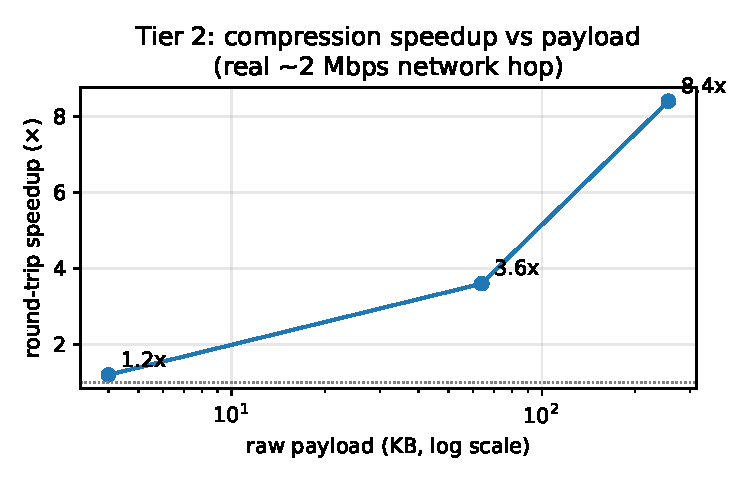
\includegraphics[width=\columnwidth]{figures/fig_tier2_crossover.pdf}
\caption{Tier~2: compression speedup grows with payload on a real bandwidth-limited link.}
\label{fig:t2}
\end{figure}

\subsection{Cluster: cold-start, warm-pool, scaling (Tier 3)}
Ephemeral CPU Jobs (ignored range, one at a time, auto-cleaned) cold-start in median $\sim$6.6\,s
($5.1$--$7.6$\,s, $n{=}5$), of which the K8s schedule$\to$container-start is $\sim$1--3\,s. A
persistent pool of $N$ queue-group workers driven from the hub (Table~\ref{tab:t3},
Fig.~\ref{fig:t3}) serves at $\sim$67\,ms per task---removing the $\sim$100$\times$ cold-start
penalty. Throughput plateaus at $\sim$930/s by two workers, and honestly so: for trivial I/O-bound
tasks the ceiling is concurrency\,$\div$\,RTT (Little's law, $64/0.067\approx 955$/s), not worker
count---one to two pods saturate the WAN link. Worker-count scaling is expected to matter for
\emph{compute-bound} tasks. Finally, batch-probe sized a BERT-base-scale encoder to batch 204 on a
GV100 and the burst ran at \textbf{94.4\% mean / 100\% peak GPU utilization} at a safe
61$^\circ$C---far above the $>$40\% policy expectation. (The batch is bounded by a safety-capped
search, not device memory; the utilization is the result.)

\begin{table}[t]\centering\caption{Tier~3 warm-pool + scaling (1\,KB tasks, concurrency 64).}\label{tab:t3}
\begin{tabular}{rrrr}\toprule
workers & throughput & p50 & p99 \\\midrule
1 & 782/s & 71\,ms & 113\,ms \\
2 & 924/s & 68\,ms & 80\,ms \\
4 & 936/s & 67\,ms & 78\,ms \\\bottomrule
\end{tabular}
\end{table}

\begin{figure}[t]\centering
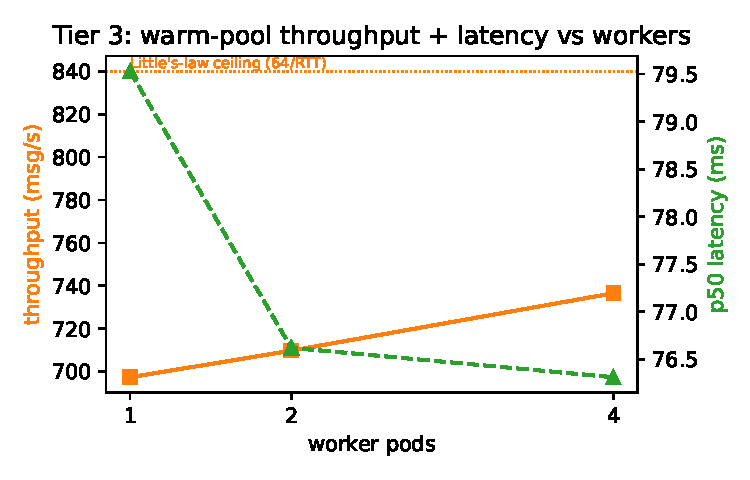
\includegraphics[width=\columnwidth]{figures/fig_tier3_scaling.pdf}
\caption{Tier~3: warm-pool throughput and latency vs.\ workers; throughput is bounded by
concurrency$\div$RTT, not pod count, for trivial tasks.}\label{fig:t3}
\end{figure}

\subsection{Admission control: goodput vs.\ politeness}\label{sec:eval-admission}
The fabric's politeness claim rests on the controller pacing concurrency to a
budget rather than grabbing all it can. We test this directly on a controlled,
variance-free testbed (local-process GPU/CPU workers; pre-registered hypotheses,
randomized interleaved trial order, four repeats) comparing three submission
policies against a self-imposed politeness budget $C$: \emph{naive} (submit up to
the hard cap), \emph{static} (fixed rate), and the controller's completion-gated
\emph{AIMD} admission. We report goodput and the over-budget fraction $\rho$
(epochs with concurrency $>C$); Table~\ref{tab:admission} and
Fig.~\ref{fig:admission} summarize.

\begin{table}[t]\centering\caption{Admission policies vs.\ a politeness budget $C$
(mean\,$\pm$\,95\% CI, 4 reps). AIMD holds the budget ($\rho{=}0$) at
$1.7$--$3.2\times$ static's goodput, and matches naive's goodput without
over-admitting.}\label{tab:admission}
\begin{tabular}{llcc}\toprule
scale & policy & goodput (tasks/s) & over-budget $\rho$ \\\midrule
GPU            & naive  & $0.0538\pm0.0003$ & $0.54$ \\
$C{=}2$        & aimd   & $0.0539\pm0.0001$ & $0.00$ \\
               & static & $0.0313\pm0.0000$ & $0.00$ \\\midrule
CPU            & naive  & $0.578\pm0.006$   & $0.95$ \\
$C{=}8$        & aimd   & $0.293\pm0.003$   & $0.00$ \\
               & static & $0.092\pm0.000$   & $0.00$ \\\bottomrule
\end{tabular}
\end{table}

\begin{figure}[t]\centering
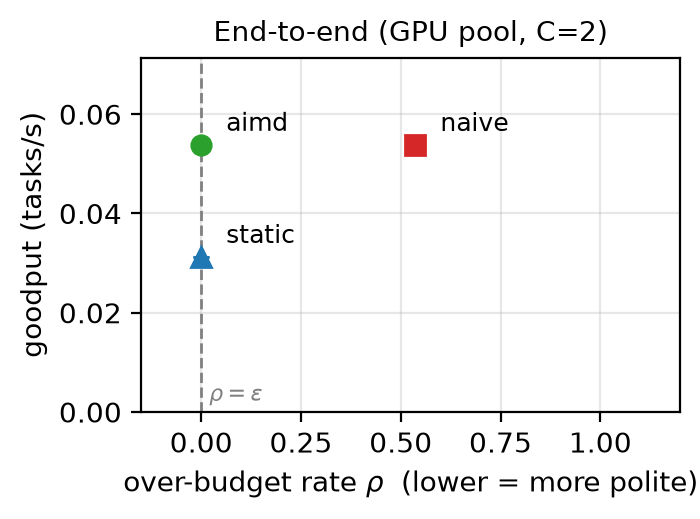
\includegraphics[width=0.84\columnwidth]{figures/pareto_gpu.png}
\caption{Goodput vs.\ over-budget $\rho$ (GPU pool, $C{=}2$). AIMD attains the
greedy policy's goodput at $\rho{=}0$ and dominates static; naive buys throughput
only by over-admitting.}\label{fig:admission}
\end{figure}

AIMD is the polite-efficient point: it holds the budget exactly ($\rho{=}0$ at
both scales) while delivering $1.72\times$ (GPU) and $3.18\times$ (CPU) static's
goodput, and it matches naive's goodput without ever exceeding the budget. naive
achieves its goodput only by over-admitting ($\rho{=}0.54$/$0.95$). Both
pre-registered hypotheses hold with disjoint CIs. \emph{Scope:} this isolates the
admission \emph{policy} on a controlled node; the full pod path
(controller$\to$node-targeted GPU worker$\to$federated result) is separately
verified end-to-end on NRP. The budget above is self-imposed---the \emph{abundance}
case; next we drive it with a real competing tenant.

\emph{Under real contention.} The sharper test is \emph{scarcity}, where a
neighbour actually contests capacity. On the two-GV100 Atlas node a competing
tenant occupies $c(t)$ of the $C{=}2$ GPUs on a fixed profile, so available
capacity $a(t){=}C{-}c(t)$ is exogenous and \emph{measured} by the prober (a
per-GPU process census); we also track \emph{harm to the neighbour}---its completed
work relative to undisturbed. Table~\ref{tab:contended} and Fig.~\ref{fig:contended}
report it (pre-registered, four seeds, randomized interleaving). Under
\emph{structured} contention (a square wave, modelling scheduled load) AIMD is the
polite-efficient \emph{knee}: $1.41\times$ static's goodput at a quarter of naive's
over-admission, while sparing the neighbour ($76\%$ of its throughput kept vs
naive's $62\%$)---naive's extra goodput is bought entirely by stealing $38\%$ of the
competitor's work. Under \emph{memoryless} contention (Poisson) AIMD breaks even
with static and over-admits more: capacity now varies faster than the prober's
detection delay, so feedback cannot track. We report this null---adaptive admission
pays when a neighbour's load has structure, and one should fall back to a fixed
budget when it does not. The micro tier (batch-probe's thermal controller,
\S\ref{sec:bp}) ran live throughout; on the GPU it throttled $>\!90\%$ of epochs
and, on this shared node, found the co-tenant thermal baseline ($\sim$$77^\circ$C)
a floor self-throttling cannot undercut---politeness extends even to heat.

\begin{table}[t]\centering\caption{Admission under real contention on
$2{\times}$GV100 ($C{=}2$; 4 seeds, mean\,$\pm$\,95\% CI). ``kept'' $=$ competitor
throughput retained ($1{=}$undisturbed). Structured (square): AIMD is the
polite-efficient knee. Memoryless (poisson): feedback breaks even with static---a
pre-registered null.}\label{tab:contended}
\begin{tabular}{llccc}\toprule
contention & policy & goodput (tasks/s) & $\rho$ & kept \\\midrule
\multirow{3}{*}{square}
 & naive  & $0.101\pm0.002$ & $0.64$ & $0.62$ \\
 & aimd   & $0.091\pm0.000$ & $0.15$ & $0.76$ \\
 & static & $0.064\pm0.000$ & $0.11$ & $0.89$ \\\midrule
\multirow{3}{*}{poisson}
 & naive  & $0.096\pm0.002$ & $0.85$ & $0.62$ \\
 & aimd   & $0.062\pm0.006$ & $0.30$ & $0.55$ \\
 & static & $0.064\pm0.000$ & $0.22$ & $0.79$ \\\bottomrule
\end{tabular}
\end{table}

\begin{figure}[t]\centering
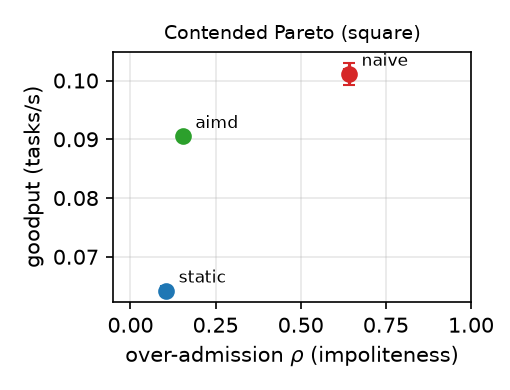
\includegraphics[width=0.49\columnwidth]{figures/pareto_contended_square.png}\hfill
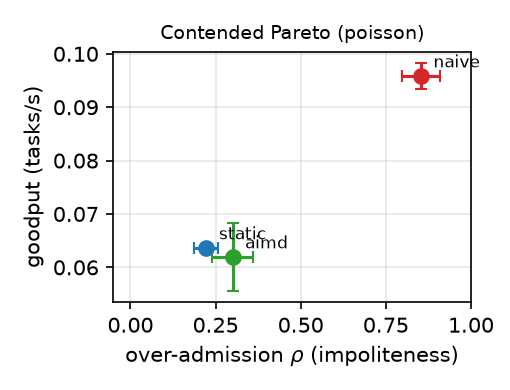
\includegraphics[width=0.49\columnwidth]{figures/pareto_contended_poisson.png}
\caption{Contended goodput--politeness frontier (lower-right is better).
\emph{Left} (square, structured): AIMD is the polite-efficient knee. \emph{Right}
(poisson, memoryless): feedback collapses onto static.}\label{fig:contended}
\end{figure}

\subsection{Positioning against task frameworks}\label{sec:eval-frameworks}
To place the fabric among general task engines, we ran the \emph{same} warm-pool workload---MiniLM
embedding on one GV100---through Ray, Dask, a raw \texttt{ProcessPoolExecutor}, and our NATS warm
pool, all same-node and warm, each driven by its \emph{native} client (Python for the first three;
the Go \texttt{nats.go} client for the pool, matching nats-bursting's Go control plane). We report
per-task \emph{dispatch latency} (a tiny round-trip isolating fabric overhead) and saturated
\emph{throughput} at four warm workers (Table~\ref{tab:frameworks}). Driven concurrently, the pool
reaches the GPU-bound ceiling---$9.4$k\,docs/s at four workers, scaling to $14.9$k at
eight---competitive with the in-process engines (Ray $9.8$k, ProcessPool $9.0$k) and far above Dask
($1.1$k); its pure-fabric ceiling (a near-empty task) is $8.3$k\,req/s. (A first-draft single-client
Python \texttt{asyncio} driver under-saturated the pool at $0.9$k\,docs/s and did not scale with
workers---a harness limit, not the bus, whose pure-fabric rate is ${>}500\times$ higher.)

nats-bursting's dispatch latency ($0.9$\,ms p50, Go client) is competitive: on par with
\texttt{ProcessPoolExecutor} ($1.0$\,ms), under Ray ($2.3$\,ms), and an order of magnitude below Dask
($13.9$\,ms). But raw dispatch is not the contribution: Ray, Dask, Parsl and Globus Compute/funcX are
mature task engines we do not try to beat. What none of them carries is a \emph{host politeness budget}, an \emph{inbound-restricted WAN
leaf-federation}, or a burst that is a \emph{publish inside the event loop}. The fabric trades
generality for lower-friction, bus-native, policy-aware bursting---a different point in the design
space, not a faster scheduler.

\begin{table}[t]\centering\caption{Same-node warm-pool comparison on one GV100 (MiniLM embedding, 4
warm workers). ``disp.'' = tiny-task round-trip (fabric overhead); ``thr.'' = embedding throughput,
each system driven by its native client (Python for Ray/Dask/ProcessPool; Go \texttt{nats.go} for
nats-bursting). Parsl (HTEx) and funcX/Globus Compute characterized by design (funcX needs a hosted
authenticated endpoint). polite = host fair-use budget; WAN = inbound-restricted leaf federation;
bus = burst is an event-loop publish.}\label{tab:frameworks}
\small
\begin{tabular}{lrrccc}\toprule
fabric & disp.\ p50 & thr.\ (d/s) & polite & WAN & bus \\\midrule
\texttt{ProcessPool}   & 1.0\,ms  & 9000 & no & no & no \\
Ray                    & 2.3\,ms  & 9800 & no & no & no \\
Dask                   & 13.9\,ms & 1050 & no & no & no \\
Parsl (HTEx)           & \multicolumn{2}{c}{by design} & no & no & no \\
funcX / Globus         & \multicolumn{2}{c}{by design} & no & part & no \\
\textbf{nats-bursting} & \textbf{0.9\,ms} & \textbf{9400} & \textbf{yes} & \textbf{yes} & \textbf{yes} \\
\bottomrule
\end{tabular}
\end{table}

\begin{figure}[t]\centering
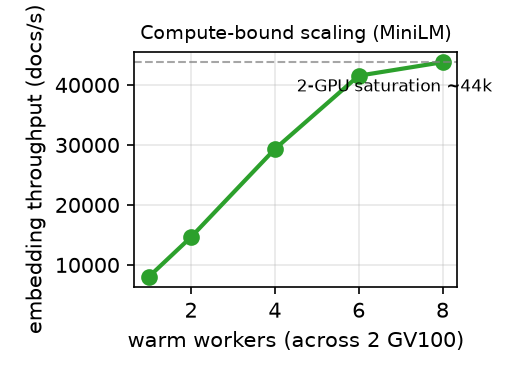
\includegraphics[width=0.74\columnwidth]{figures/embed_scaling.png}
\caption{Compute-bound scaling: MiniLM embedding throughput vs warm-worker count across two GV100s.
Unlike the I/O-bound warm-pool plateau (Fig.~\ref{fig:t3}, Little's law), a compute-bound AI
workload scales with parallelism until the GPUs saturate (${\sim}44$k\,docs/s at eight workers,
$5.4\times$ one).}\label{fig:embed-scaling}
\end{figure}

\section{Threats to validity}\label{sec:threats}
We state these so the numbers are read correctly. \textbf{Synthetic data (Tier 1):} real bge
embeddings reproduce the random numbers within 0.001; cosine remains a fidelity proxy.
\textbf{Loopback (Tier 2):} addressed by the real $\sim$2\,Mbps hop ($1.2\!\to\!8.4\times$); it is
one overlay (likely relayed) path---a characterized datacenter link would pin absolute bandwidth.
\textbf{Cold-start realism (Tier 3):} warm node + cached image + \texttt{kubectl wait} inflate the
total; the K8s breakdown isolates the cluster-side cost; warm-pool and a real NATS-join are
measured, while a cold image pull and a GPU-image run remain. \textbf{Scaling:} the plateau is
explained by Little's law, not presented as pod-count scaling; a compute-bound load is the named
next run. \textbf{Contention realism:} the contended Pareto is manufactured on a two-GPU node
($C{=}2$), not a production multi-tenant trace, and the Poisson regime marks where feedback stops
beating a fixed budget (capacity outpaces the prober's detection delay). \textbf{Portability:}
batch-probe's thermal sensing is Linux-only and its feedforward is one-sided. \textbf{Cluster citizenship:} the
harness is policy-safe by construction (ignored-range pods, $\le$4 concurrent, exit-0 Jobs, TTL +
delete cleanup, an explicit policy gate, and---above the harness---the controller's politeness
backoff).

\section{Discussion}\label{sec:discussion}
``Effective'' use is batch-probe sizing pods to high utilization (94\% measured); ``policy-safe''
is the politeness controller plus the gate, short runs, and cleanup. The deployment rule for
compression is now evidenced: compress when the link or bus is the bottleneck---a wash on a fast
LAN, a large and growing win on a real WAN-class link.

\textbf{Lessons learned.} Three points generalize. First, on a multi-tenant cluster the
\emph{usage policy is a first-class design constraint}: it shaped the politeness controller, the
ignored-range defaults, and the no-sleep worker as much as any performance goal, and a benchmark
that strays outside policy is itself a bug. Second, \emph{leaf-node federation leaks into the
application}: the durable-vs-core dispatch choice and the result webhook both exist only because
JetStream and subject interest do not cross a leaf link symmetrically---a from-scratch design that
ignored this would deadlock on the return path. Third, \emph{honest negatives beat flattering
curves}: reporting the Little's-law plateau and labeling the cold-start as warm-node/cached-image
makes the result more useful to an operator than a scaling plot that does not hold.

\textbf{When to use which shape.} An ephemeral Job costs a $\sim$6.6\,s cold start but holds no
resources between bursts---right for occasional or embarrassingly parallel work. A persistent pool
pays that once and serves at $\sim$67\,ms but occupies its slots---right for interactive or
sustained workloads, provided it is sized within policy and torn down when idle. The bus makes
switching a configuration choice, not a rewrite.

\section{Related work}
\textbf{Bursting and task frameworks.} Spilling local work to remote capacity is long-studied:
HTCondor flocking~\cite{htcondor} federates pools; Globus Compute/funcX~\cite{funcx} offers a
federated function-serving fabric; Ray~\cite{ray}, Dask~\cite{dask}, and Parsl~\cite{parsl} build
task graphs over remote workers. All treat the remote resource as an external system one submits
to and polls. Message-oriented task systems (Celery, RabbitMQ workers) put a broker between
producer and consumer, and Kubernetes-native batch layers (Kueue, Volcano) schedule Jobs beneath
the application. Two things set our approach apart: \emph{orientation}---containerized pods become
first-class subscribers on the researcher's own bus, so a burst is a publish inside the event loop
rather than a hand-off---and an explicit \emph{politeness} control loop that probes a shared,
multi-tenant cluster and backs off to yield to other tenants, which the submit-and-poll model
leaves to the user.

\textbf{Quantization and attention.} turboquant-pro builds on the random-rotation,
near-optimal-distortion line of TurboQuant~\cite{turboquant} and the broader embedding/KV-cache
quantization literature; its compute-on-codes fused decode applies online-softmax and
IO-aware attention techniques~\cite{onlinesoftmax,flashattention} in the \emph{code} domain so that
quantized values are never reconstructed (per-channel keys are reconstructed). Our paper does not propose a new codec; it
contributes a measured account of \emph{when} on-wire compression pays for the bursting use case,
and the systems integration that makes a quantized payload a transparent bus primitive.

\textbf{Resource and thermal control.} OOM-driven batch-size search is folklore; batch-probe makes
it robust (optimizer-state-aware peak-memory accounting, a unified multi-framework OOM-recovery
path). Thermal management of CPUs and accelerators is usually fixed-threshold throttling;
batch-probe instead estimates thermal state with a Kalman filter~\cite{kalman} and acts on the
\emph{predicted} trajectory, throttling parallelism before overshoot---closer to model-predictive
control than to a thermostat.

\section{Artifact availability}\label{sec:artifact}
All three projects are open and on PyPI---\texttt{nats-bursting}~\cite{natsbursting},
\texttt{turboquant-pro}~\cite{turboquantpro}, and \texttt{batch-probe}~\cite{batchprobe};
Table~\ref{tab:impl} reports their shipped size. The benchmark harness
reproduces every measurement here:
\texttt{bench\_compression.py} (Tier~1, with a real-embedding variant), \texttt{bench\_transport.py}
and the co-existing real-hop driver (Tier~2), and \texttt{bench\_cluster.py} with
\texttt{--mode cold|warm|scale} (Tier~3), the last gated behind \texttt{--i-have-checked-nrp-policy}.
Result files and a \texttt{make\_figures.py} that regenerates every figure are committed alongside.

\begin{table}[t]\centering\caption{Shipped implementation per project (importable package or
binary; excludes tests, benchmarks, and experiment scripts).}\label{tab:impl}
\begin{tabular}{llr}\toprule
project / component & language & LOC \\\midrule
nats-bursting controller & Go & 752 \\
nats-bursting client + pools & Python & 1{,}398 \\
turboquant-pro & Python (+CUDA via CuPy) & 11{,}379 \\
batch-probe & Python & 1{,}082 \\\midrule
\textbf{total} & & \textbf{14{,}611} \\\bottomrule
\end{tabular}
\end{table}

\section{Conclusion}
nats-bursting, turboquant-pro, and batch-probe form a small, composable, open pipeline that makes
a shared, containerized cluster usable from inside the event loop---effectively, and within
policy by construction. We described each system's architecture, including the politeness
controller, the compute-on-codes codec, and the Kalman-filtered thermal governor, and quantified
the composition with real measurements, threats stated and remaining runs scoped. More broadly,
the pattern---cluster pods as first-class subscribers reached over an outbound leaf link, behind a
controller that defers to its neighbors---generalizes to any Kubernetes cluster a researcher can
bridge to, and the policy-safe discipline it enforces is the right default for sharing a
multi-tenant resource.

\appendices
\section{Artifact Description (AD)}\label{sec:ad}

\subsection{Overview}
The artifact is the three open-source projects evaluated here---\texttt{nats-bursting}
(the bursting fabric), \texttt{turboquant-pro} (transport codec), and \texttt{batch-probe}
(GPU right-sizing and thermal control)---plus a self-contained benchmark harness that
regenerates every number, table, and figure in \S\ref{sec:eval}. Every reported number is
produced by this harness.

\subsection{Artifact check-list (metadata)}
\begin{itemize}\itemsep1pt
\item \textbf{Algorithms:} polite admission control (Alg.~\ref{alg:polite}); OOM-safe batch
search (Alg.~\ref{alg:probe}); random-rotation quantization; Kalman-filtered thermal control.
\item \textbf{Program:} Go~1.23 control plane; Python~3.12 client, codec, right-sizer, harness.
\item \textbf{Compilation:} \texttt{go build ./...}; Python packages install from PyPI.
\item \textbf{Data set:} synthetic fp32 vectors (dim 384/768/1024) and real
\texttt{bge-small-en-v1.5} embeddings on 20newsgroups ($n{=}3000$, dim~384), fetched by the harness.
\item \textbf{Run-time environment:} Linux; \texttt{nats-server} with JetStream;
\texttt{kubectl}/client-go with credentials to a Kubernetes cluster for Tier~3.
\item \textbf{Hardware:} Tiers~1--2 run on any CPU host; Tier~3 and GPU right-sizing need an
NVIDIA GPU (measured on a GV100 32\,GB) and a shared cluster (measured on NRP Nautilus).
\item \textbf{Metrics:} compression ratio and reconstruction cosine; round-trip p50/p99 and
throughput; Job cold-start; warm-pool latency/throughput; GPU utilization; admission goodput
and over-budget fraction~$\rho$.
\item \textbf{Output:} JSON result files under \texttt{benchmarks/}; regenerated figures under
\texttt{paper/figures/}.
\item \textbf{Disk / setup / run:} $<$1\,GB; setup $<$10\,min; Tiers~1--2 run in minutes; Tier~3
depends on cluster scheduling.
\item \textbf{Publicly available:} yes---as PyPI packages and at
\texttt{github.com/ahb-sjsu} (repositories \texttt{nats-bursting}, \texttt{turboquant-pro},
\texttt{batch-probe}).
\item \textbf{License:} MIT (all three projects).
\item \textbf{Archived DOI:} \texttt{nats-bursting} 10.5281/zenodo.20660069;
\texttt{turboquant-pro} 10.5281/zenodo.20660087; \texttt{batch-probe} 10.5281/zenodo.21095035
(concept DOIs; always resolve to the latest release).
\end{itemize}

\subsection{How to access, and dependencies}
The projects are on PyPI and GitHub (above). \textbf{Hardware:} Tiers~1--2 need only a CPU host;
Tier~3 and the GPU-utilization result need an NVIDIA GPU and \texttt{kubectl} access to a shared
cluster; the real-hop transport result needs a bandwidth-constrained WAN path between client and
server. \textbf{Software:} Linux, Python~3.12, Go~1.23, \texttt{nats-server} (with JetStream for the
durable path), NumPy, and PyTorch for the GPU right-sizing trial.

\subsection{Installation}
\begin{verbatim}
pip install nats-bursting turboquant-pro \
            batch-probe numpy
git clone \
 https://github.com/ahb-sjsu/nats-bursting
cd nats-bursting && go build ./...
\end{verbatim}

\subsection{Experiment workflow}
Each reported result maps to one command; \texttt{make\_figures.py} regenerates the figures from
the committed JSON.
\begin{itemize}\itemsep1pt
\item \textbf{Tier~1 (Fig.~\ref{fig:t1}):} \texttt{python benchmarks/bench\_compression.py}
$\rightarrow$ \texttt{results\_compression.json} (real-embedding variant:
\texttt{results\_compression\_real.json}).
\item \textbf{Tier~2 (Tables~\ref{tab:t2lo},~\ref{tab:t2}, Fig.~\ref{fig:t2}):} start a bus
(\texttt{docker run -p 4222:4222 nats}), then \texttt{python benchmarks/bench\_transport.py
[-{}-compress]}; the real-hop driver writes \texttt{results\_transport\_realhop.json}.
\item \textbf{Tier~3 (Table~\ref{tab:t3}, Fig.~\ref{fig:t3}):} \texttt{python
benchmarks/bench\_cluster.py -{}-mode cold|warm|scale -{}-i-have-checked-nrp-policy} $\rightarrow$
\texttt{results\_cluster\_pool.json}; GPU right-sizing writes \texttt{results\_batchprobe.json}.
\item \textbf{Admission (Table~\ref{tab:admission}, Fig.~\ref{fig:admission}):} the pre-registered
harness in \texttt{benchmarks/infocom/} (\texttt{run.py}, \texttt{e8\_local.py},
\texttt{multiseed.py}, \texttt{aggregate.py}); protocol and pre-registration in
\texttt{E8\_PROTOCOL.md} and \texttt{E8\_PREREG.md}.
\item \textbf{Figures:} \texttt{python paper/\allowbreak figures/\allowbreak make\_figures.py}.
\end{itemize}

\subsection{Evaluation and expected results}
Hardware permitting, the harness reproduces: Tier~1 ratios $7.9/10.4/15.5\times$ at $4/3/2$-bit with
cosine $0.995/0.978/0.94$, real embeddings matching within $0.001$; Tier~2 up to $8.4\times$
round-trip speedup at 256\,KB over the $\sim$2\,Mbps hop; Tier~3 median cold-start $\sim$6.6\,s,
warm-pool $\sim$67\,ms, throughput plateau $\sim$930/s (the Little's-law bound); GPU right-sizing
$\approx$94\% utilization on a GV100; and AIMD admission at $\rho{=}0$ with $1.7$--$3.2\times$
static's goodput. Absolute latencies, cold-start, and utilization depend on the cluster, WAN path,
and GPU model; the qualitative results (compression win grows with payload, warm pool removes the
cold-start penalty, AIMD holds the budget) are hardware-independent.

\subsection{Notes}
Tier~3 refuses to run without \texttt{-{}-i-have-checked-nrp-policy} and uses ignored-range pods
($\le$4 concurrent, cpu=1/mem=2\,GiB, exit-0 Jobs, TTL${+}$delete) to respect shared-cluster policy.
Thermal sensing in \texttt{batch-probe} is Linux-only. The real-hop bandwidth is one overlay path
(likely relayed); a cold image pull and a full GPU-image cluster run are not yet measured
(\S\ref{sec:threats}).

\bibliographystyle{IEEEtran}
\bibliography{paper}

\end{document}
